\documentclass[10pt,twocolumn,letterpaper]{article}

\usepackage{cvpr}
\usepackage{times}
\usepackage{epsfig}
\usepackage{graphicx}
\usepackage{amsmath}
\usepackage{amssymb}

\usepackage{url}

% Include other packages here, before hyperref.
\usepackage{algorithm}
\usepackage{algpseudocode}
% If you comment hyperref and then uncomment it, you should delete
% egpaper.aux before re-running latex.  (Or just hit 'q' on the first latex
% run, let it finish, and you should be clear).
%\usepackage[pagebackref=true,breaklinks=true,letterpaper=true,colorlinks,bookmarks=false]{hyperref}

\cvprfinalcopy % *** Uncomment this line for the final submission

\def\cvprPaperID{****} % *** Enter the CVPR Paper ID here
\def\httilde{\mbox{\tt\raisebox{-.5ex}{\symbol{126}}}}

% Pages are numbered in submission mode, and unnumbered in camera-ready
\ifcvprfinal\pagestyle{empty}\fi
\begin{document}

\title{Comparison between a sequential and a distributed version of a Twitter sentiment analysis tool}

\author{
    Emilio Cecchini \\
    {\tt\small emilio.cecchini@stud.unifi.it}
}

\maketitle
\thispagestyle{empty}

\begin{abstract}
In this paper I will analyze the advantages in speed and efficiency obtainable in implementing a Twitter sentiment analysis tool with Hadoop. The main goal of this study is not to build a perfect classifier, but it is instead to show the speedup that you can get using a distributed algorithm versus a sequential version. To build the sentiment classifier the library LingPipe is used, so the details of that classifier will be ignored. The distributed version is written in Hadoop with the MapReduce framework.
\end{abstract}

\section{Introduction}

Sentiment analysis involves classifying opinions in text into categories like \textit{positive} or \textit{negative} often with an implicit category of \textit{neutral}. In this project, for simplicity, we will ignore the \textit{neutral} category. All the entire part of building the classifier and getting results out of it is done with the LingPipe library, that is a Java library to perform machine learning tasks such as text classification and natural language processing.

First of all there is a \textit{training} phase, where the model is trained to recognize a tweet as negative or positive. This phase is only implemented in a sequential version. Once the model is built and trained, there is the \textit{classification} phase, where many unclassified tweets are passed as input to the model. This phase is implemented in two different versions: a sequential version and a distributed version in Hadoop with the MapReduce framework.

\section{Training}

The training process is done with a dataset containing tweets already classified. The model reads the tweet texts and their sentiment and try to learn how to perform the classification.

The process of training the model must be computed in a sequential way because every tweet and its associated sentiment must be processed by the same unique model. A parallel version could be hypothetical possible but in that case reading and processing the tweet must be encapsulated in a critical section and therefore all the advantages of parallelization would be lost.

Thanks to the LingPipe library, the algorithm of training the model is straightforward:

\begin{algorithm}[H]
\caption{Training the model}
\textbf{Input:} a list of tweets $T$ with text and sentiment. \\
\begin{algorithmic}
    \State $m$ = initializeModel()
    \For{each $t \in T$}
        \State handle($m$, $t$)
    \EndFor
    \State saveModel($m$)

\end{algorithmic}
\end{algorithm}

The function \verb"saveModel()" save the model in a file so that it can be loaded later by a classifier to perform a classification.

\section{Classification}

The classification phase can be performed in a distributed way, so I have implemented a sequential version and a distributed version in Hadoop.

\subsection{Sequential version}

With the LingPipe library it is very easy to implement a sequential algorithm that classify tweets.

The first thing to do is to load the trained model. This process may take a long time if the model has been trained with a very large dataset. Loading the model can not be parallelized, so it is suggested to keep the file as small as possible to prevent it to become the bottleneck of the program.

After loading the model, the program iterates over the tweet texts and uses the classifier to predict their sentiment. During the iteration, the program keep tracks of the number of negative tweets as well as the number of positive tweets with two counters. The output of this algorithm are the two counters from which the general sentiment can be derived.

\begin{algorithm}[H]
\caption{Sequential classification}
\textbf{Input:} a list of tweets $T$ with text only. \\
\textbf{Output:} two values $p, n \in \mathbb{N}$ that are the number of tweets classified as positives or negatives respectively. \\
\begin{algorithmic}

    \State $m$ = loadModel()
    \State $p$ = 0
    \State $n$ = 0
    \For{each tweet $t$}
        \State $s$ = classify($m$, $t$)
        \If{isPositiveSentiment($s$)}
            \State $p$ = $p$ + 1
        \Else
            \State $n$ = $n$ + 1
        \EndIf
    \EndFor
    \State \Return $p$, $n$

\end{algorithmic}
\end{algorithm}

\subsection{Distributed version}

The classification process can be improved by implementing a distributed algorithm. This project uses Hadoop with its \textit{Hadoop Distributed File System} (HDFS) in order to better handle large amounts of data.

The distributed algorithm is implemented with the \textit{MapReduce} framework, that is a programming model for processing and generating big data sets on a cluster of computers. A MapReduce program is composed by a \textit{map} phase, which performs a filtering operation of the input data, and a \textit{reduce} phase, which collects the results of the map function and generate an output. The map function processes each element of the input and returns a value associated with a key. The reduce function takes as input the keys returned by the map function and their associated values and then it combines them in a single value.

In order to perform the classification of a tweet the model must first be loaded. This implementation exploits the \textit{Distributed Cache} tool to make the file where the model is stored accessible to all the map tasks. The Distributed Cache is a read-only data structure from which each application in the MapReduce framework can read files. Each map task loads its own model so there are not synchronization issues such as race conditions.

Once the model is loaded from its file we can perform the map phase, which consists of mapping each tweet text to its classified sentiment.

\begin{algorithm}[H]
\caption{Map function}
\textbf{Input:} a trained model $m$, a tweet text $t$ \\
\textbf{Output:} a key $k$ and a value $v = 1$ \\
\begin{algorithmic}
    \State s = classify($m$, $t$)
    \If{isPositiveSentiment($s$)}
        \State $k$ = \textit{positives}
    \Else
        \State $k$ = \textit{negatives}
    \EndIf
    \State \Return $k$, 1

\end{algorithmic}
\end{algorithm}

As you can see, the map function is very similar to a single iteration of the sequential algorithm. The input for the map function is a single tweet text, this text is classified with the previously loaded model and then the output key is generated depending on the classified sentiment. There could be only two different output keys: \textit{positives} if the tweet has been classified as positive and \textit{negatives} if the tweet has been classified as negative.

The reduce phase is quite straightforward. It takes as input the key, which as already explained can be \textit{positives} or \textit{negatives} and a list of as many ones as many tweets have been classified in that category.

\begin{algorithm}[H]
\caption{Reduce function}
\textbf{Input:} a key $k$ and a list $V$ of values $v = 1$ \\
\textbf{Output:} a key $k$ and a value $c$ \\
\begin{algorithmic}
    \State $c$ = 0
    \For{each element in $v \in V$}
        \State c = c + 1
    \EndFor
    \State \Return $k$, $c$
\end{algorithmic}
\end{algorithm}

The only thing that the reduce function has to do is to count the number of elements that are in the list associated with the input key.

Since the keys that the mapper passes to the reducer are always two (\textit{positive} or \textit{negatives}), the number of reducers can be specified at compilation time to two. Moreover, to optimize the operations of dispatching the mapper output, a \textit{partition} function is implemented. The purpose of this function is to assign the output key of a map function to a specific reducer. Since we have set the number of reducers to two, the output of this function is 1 or 0 dependending if the key is \textit{positives} or \textit{negatives}.

\begin{algorithm}[H]
\caption{Partion function}
\textbf{Input:} a key $k$ \\
\textbf{Output:} a value $v$ \\
\begin{algorithmic}
    \If{$k$ == "positives"}
        \State \Return 1
    \ElsIf{$k$ == "negatives"}
        \State \Return 0
    \Else
        \State \Return -1 \Comment{Error}
    \EndIf
\end{algorithmic}
\end{algorithm}

In this way we have one reducer that counts the number of tweets classified as positives and another reducer which counts the number of tweets classified as negatives.

\section{Speedup analysis}

To compare the performance of a sequential algorithm with a parallel version, the main measure used is the \textit{speedup}, that is the ration between the execution time of the sequential version and the execution time of the parallel version with the same input.

\begin{align}
S = \dfrac{t_S}{t_P}
\end{align}

Ideally, the speedup should be the number of processor used to perform the parallel version. For a distributed algorithm, it should be the number of nodes in the cluster. In this section we report the results of some experiments in order to analyze the speedup of the classification algorithm in its two versions: sequential and distributed.

The inputs for these experiments are some text files containing the tweet texts. The size of a single text file is about the size of a HDFS block, that is 128 MB by default. This make it easier to control the number of splits into which the input will be divided. In order to see the trend of the speedup, we tested the distributed algorithm in a cluster with a different number of nodes, more precisely from two to five nodes. Each node has an Intel Haswell CPU with four cores and 8 GB of RAM.

In this plot there are the speedups obtained with an input consisting of a single text file, that is a single HDFS block.

\begin{figure}[H]
\centering
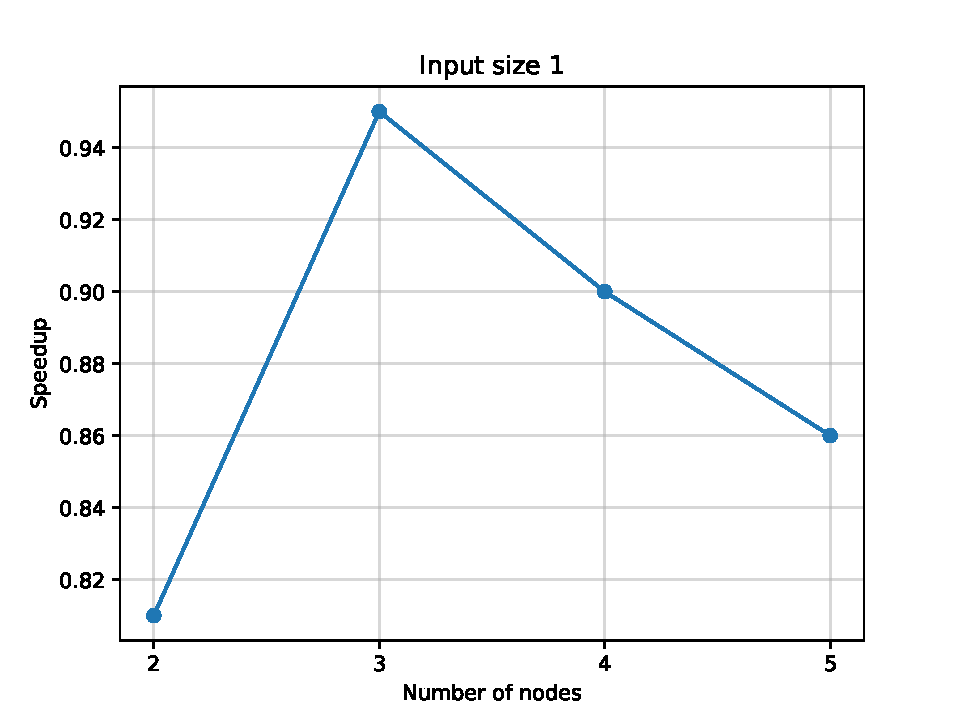
\includegraphics[width=3.2in]{fig/speedup1}
\end{figure}

As you can see, with an input of only one file, the distributed version is slower than the sequential algorithm because the speedup is minor than one. The reason of that is because the time spent in managing the various tasks and moving the data in the distributed environment is too much to get an improvement in the overall execution time.

Here we report the speedups with an input of five files, that are five HDFS blocks.

\begin{figure}[H]
\centering
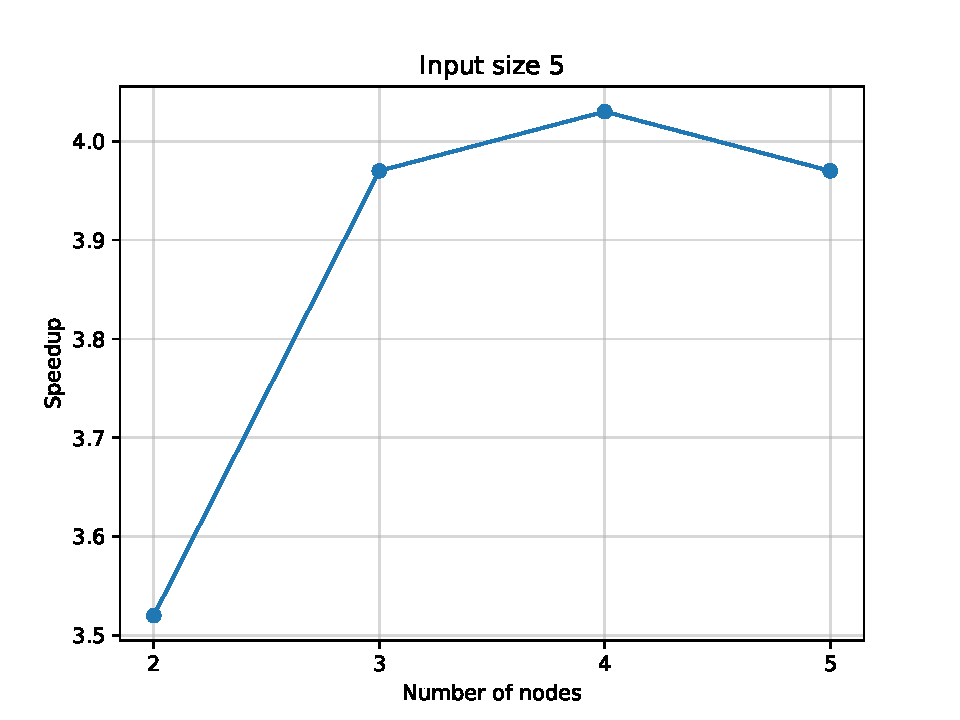
\includegraphics[width=3.2in]{fig/speedup5}
\end{figure}

Increasing the size of the input we can see a big improvements in the performances. With only two nodes you have a speedup of 3.5, with three, four and five nodes the speedup stabilizes around 4. It means that with an input of that size, that is five HDFS blocks, until three nodes you get a \textit{super-linear} speedup, with four nodes you get a \textit{linear} speedup and with five nodes you get a \textit{sub-linear} speedup.

Here we report the speedups with an input of ten files, that are ten HDFS blocks.

\begin{figure}[H]
\centering
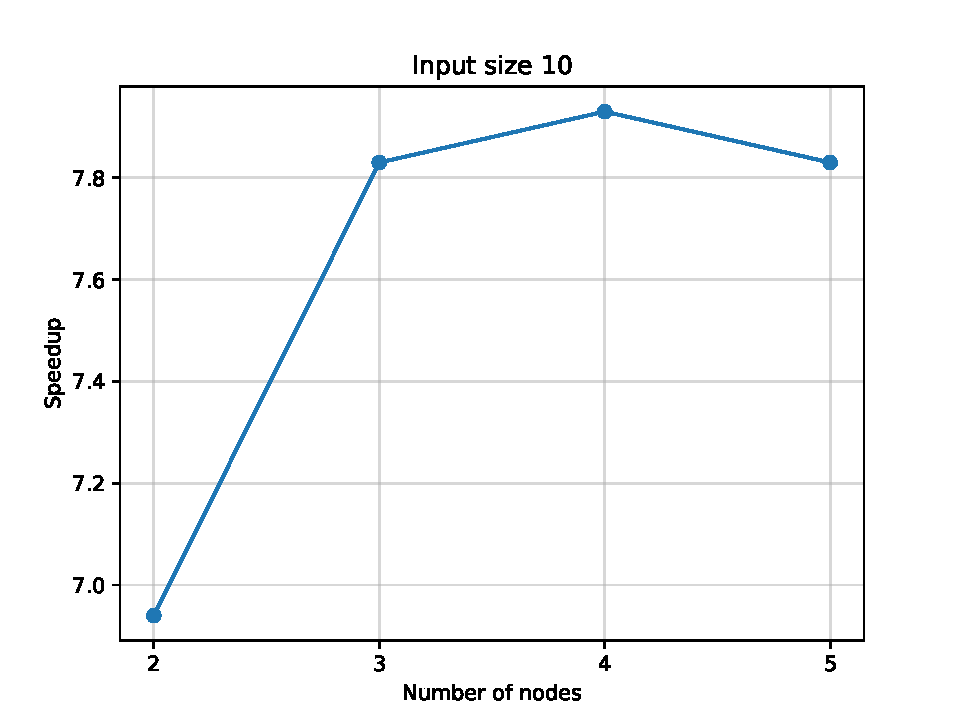
\includegraphics[width=3.2in]{fig/speedup10}
\end{figure}

We can notice that the trends is the same as in the previous plot, but the obtained speedups are higher.

Here we report the speedups with an input of twenty files, that are twenty HDFS blocks.

\begin{figure}[H]
\centering
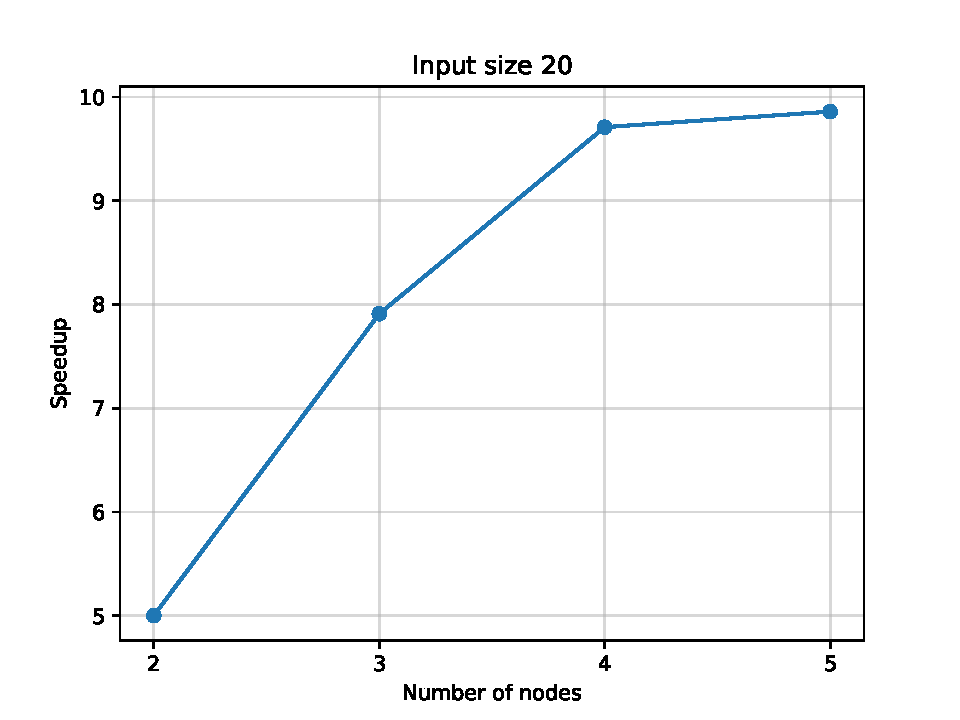
\includegraphics[width=3.2in]{fig/speedup20}
\end{figure}

With an input size of about 2.5 GB we get better performances with a larger number of nodes, such as four or five.

From these simple experiments we can confirm that Hadoop is designed to work with big data, because if the input size is too small we have a lot of overhead due to tasks management. Apart from the first case, where we passed only a single file to the classifier, the speedups are always super-linear, that means that the speedup is alway greater then the number of nodes in the clusters.

\end{document}
